\documentclass[a4paper,11pt]{article}
\usepackage{a4wide,amsmath,ngerman,url,graphicx}
\usepackage[utf8]{inputenc}
\parskip4pt
\parindent0pt

\newcommand{\br}[1]{\left(#1\right)}
\newcommand{\erf}{\mathrm{erf}}
\newcommand{\m}{\cdot}

\title{Analyse der Coronastatistiken} 
\author{Hans-Gert Gräbe, Leipzig}
\date{Version vom 1. April 2020}

\begin{document}
\maketitle

Dieser Text bezieht sich auf die im Verzeichnis
\url{http://leipzig-data.de/demo/Corona-20/Code} verfügbaren Materialien.

\section{Datenbasis}

Als Datenbasis werden die von der John Hopkins Universität (JHU) als
Excel-Datei veröffentlichten Daten\footnote{Siehe deren github-Projekt
  \url{https://github.com/CSSEGISandData/COVID-19}.} zur Entwicklung der
weltweit registrierten Covid-19-Fälle (Stand 28.03.2020) verwendet. Die
Statistik listet pro Land und Tag die kumulierte Zahl der Infizierten, die
Zahl der Genesenen und die Zahl der Todesfälle auf.

\section{Installation} 

Zunächst muss das git Repo der JHU lokal geklont und der Pfad im Skript
\texttt{extractData.pl} eingetragen werden.  Die Daten werden für ausgewählte
Länder mit diesem Perl-Skript für die weitere Verarbeitung aufbereitet und in
einer Datei \texttt{BasicData.txt} gespeichert, um dann mit dem freien CAS
\emph{Maxima}\footnote{Siehe dazu \url{http://maxima.sourceforge.net/de/}, das
  CAS ist in Linux-Distributionen über den Paketmanager leicht zu
  installieren.} weiterverarbeitet zu werden.

\section{Datentransformation}

In der Datei \texttt{BasicData.txt} sind die Daten für jedes der ausgewählten
Länder in einem Array mit drei Einträgen (infected, recovered, dead)
gespeichert, die im Maxima-Skript \texttt{skript.m}\footnote{Dies ist eine
  reine Textdatei mit Code-Schnipseln, die nicht für den Batchbetrieb
  konzipiert ist.} in einer Funktion \texttt{getland(Land)} zunächst einmal zu
Paaren $(t,y_t)$ ergänzt werden, wobei $t$ für den Tag des Jahres
($0=01.01.2020$) und $y_t$ für die Zahl der Fälle aus dem jeweiligen Record
stehen.

\section{Fitting}

Alle Grafiken zu Prognosen der Daten, die ich bisher gesehen habe, gehen von
einer „Glockenkurve“ aus.  Das kann natürlich nur die Entwicklung der Zuwächse
pro Tag abbilden, die aus den kumulierten Daten zunächst als $d_t=y_t-y_{t-1}$
extrahiert werden müssen. Dies geschieht mit der im Skript definierten
Maxima-Funktion \texttt{Delta}.

Zur Abschätzung des Verlaufs längs einer Glockenkurve wird üblicherweise die
Statistikfunktion $C\m\exp\br{-\br{\frac{t-m}{s}}^2}$ verwendet, die ich als
Kurvenschar $f(t)=\exp\br{c-\br{\frac{t-m}{s}}^2}$ zur Parameterschätzung auf
die Daten $(t,d_t)$ ansetze.  Die (kumulierten) Originaldaten $(t,y_t)$
sollten dann auf die Funktion
\begin{align*}
  h(x)&=\int_0^x{\exp\br{c-\br{\frac{t-m}{s}}^2}}\,dt\\ &=\exp(c)\m s\m
  \int_{-\frac{m}{s}}^{\frac{x-m}{s}}{\exp\br{-u^2}}\,du\\ &=\frac12 \sqrt{\pi}\m
  \exp(c)\m s\m \br{\erf\br{\frac{x-m}{s}}+ \erf\br{\frac{m}{s}}}
\end{align*}
matchen, wobei $\erf(x)$ für die Fehlerfunktion steht und im zweiten Schritt
die Variablensubstitution $u=\frac{x-m}{s}$ mit $du=s\m dt$ erfolgte.

Nun sind die Parameter $(c,s,m)$ dieser Kurvenschar so zu fitten, dass die
ermittelte Kurve besonders gut auf die Daten passt.  In \emph{Maxima} kann
dazu das Paket \emph{lsquares} verwendet werden.  

Wir hätten natürlich auch versuchen können, die Originaldaten auf die Schar
$h(t)$ zu fitten, aber Fitting auf nicht polynomialen Kurvenscharen ist eine
schwierige und numerisch wenig stabile Angelegenheit, bei der Maxima schnell
an seine Grenzen kommt (und die Ergebnisse anderer CAS sehr genau zu
analysieren sind, da die Fitting-Ergebnisse stark von Startwerten der dabei
eingesetzten Verfahren abhängen).

\emph{Maxima} kommt auch beim Fittung der Schar $f(t)$ zu keinem Ergebnis.
Einen einfacheren, nämlich quadratischen Zusammenhang
$g(t)=c-\br{\frac{t-m}{s}}^2$ erhält man, wenn man zu Paaren $(t,\log(d_t))$
übergeht.  Damit lassen sich dann die Fittingparameter stabil berechnen. Dafür
müssen aber vorher Datenpunkte aussortiert werden, wo $d_t=0$ ist.

Genrell kann es sinnvoll sein, für ein gutes Fitting Datenpunkte unterhalb
einer Schwelle auszusortieren. Eine solche Schwelle ist als weiterer Parameter
im Skript in der Funktion \texttt{FittingDelta} vorgesehen. Für die meisten
Datensätze ist die Schwelle 50 eine gute Wahl\footnote{Es ist zu beachten,
  dass die Schwelle die Dateninkremente $d_t$ auswertet, nicht die kumulierten
  Daten $y_t$.  Ein kleines Land wie Österreich bereitet hier besondere
  Schwierigkeiten.}.

Details sind im Skript \texttt{skript.m} zu finden.

Weitere Versuche, etwa mit einer Schar von Logistik-Funktionen, lassen sich
mit dem CAS Maxima nicht erfolgreich zu Ende bringen. 

\section{Ergebnisse}

Die Rechnungen werden für jedes der Länder nun wie folgt ausgeführt:
\begin{enumerate}
\item Fasse mit \texttt{getData} die drei Datensätze für das Land als Tripel
  von Listen $(t,y_t)$ zusammen. 
\item Berechne für jeden der drei Datensätze mit \texttt{getFittingFunctions}
  das Fitting auf $(t,\log(d_t))$ gegen die Funktion $g(t)$ und verwende das
  gefundene Fitting, um Funktionen $h_1(t)$ (für infected), $h_2(t)$ (für
  recovered) und $h_3(t)$ (für dead) zu schätzen. 
\item Erzeuge daraus einen Plot, welcher die Datenpunkte und die drei Kurven
  in verschiedenen Farben (rot für infected, grün für recovered, blau für
  dead) ausgibt.  
\end{enumerate}
Bei erfolgreichem Fitting ist eine gute Übereinstimmung der jeweiligen Kurve
\begin{gather*}
  h(t)=A\br{\erf\br{B(t-m)+1}}
\end{gather*}
mit den Datenpunkten zu verzeichnen.  Die berechneten Parameter haben folgende
Bedeutung:
\begin{itemize}
\item $m$ -- Tag, an dem die Spitze in den Inkrementdaten erreicht ist.
\item $B=\frac{1}{s}$ -- $[m-s \ldots m+s]$ ist das kritische Intervall.
\item $2*A$ -- Zahl der am Ende insgesamt betroffenen Personen. 
\end{itemize}

Auf der Basis der Daten vom 29.03.2020 lassen sich folgende Szenarien (!) für
die Länder Deutschland, Italien, Spanien und Österreich erstellen, siehe auch
die Abbildungen.

\begin{center}
  \begin{tabular}{|l|r|r|r|}\hline
    & $m$ & $s$ & $2A$ \\\hline
    \multicolumn{4}{|c|}{\bf Deutschland}\\\hline
    infected   & 94 & 14 & 171274\\
    recovered  & 90 &  5 &  20730\\
    dead       & 95 & 10 &   2624\\\hline
    \multicolumn{4}{|c|}{\bf Italien}\\\hline
    infected   & 85 & 15 & 144893\\
    recovered  & 94 & 18 &  39909\\
    dead       & 90 & 15 &  22893\\\hline
    \multicolumn{4}{|c|}{\bf Spanien}\\\hline
    infected   & 89 & 12 & 156889\\
    recovered  & \multicolumn{3}{|c|}{bad fitting}\\
    dead       & 95 & 12 &  23378\\\hline
    \multicolumn{4}{|c|}{\bf Österreich}\\\hline
    infected   & 88 & 11 &  13747\\
    recovered  & \multicolumn{3}{|c|}{bad fitting}\\
    dead       & \multicolumn{3}{|c|}{bad fitting}\\\hline
  \end{tabular}
\end{center}
Natürlich müsste am Ende die Zahl der Infizierten mit der Summe der Zahlen der
Genesenen und der Verstorbenen übereinstimmen.  Die Schätzungen sind von einer
solchen Invarianzforderung weit entfernt, was ein Licht auf die prognostische
Qualität der Schätzungen für die weitere Zukunft (drei bis vier Wochen, also
30 Tage) wirft.

\begin{figure}
  \begin{center}
    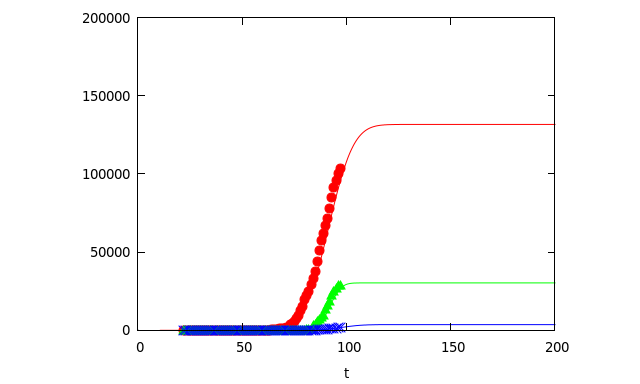
\includegraphics[width=.8\textwidth]{Germany.png}
    \caption{Szenario für Deutschland (82.9 Mio. Einwohner)}
  \end{center}
\end{figure}
\begin{figure}
  \begin{center}
  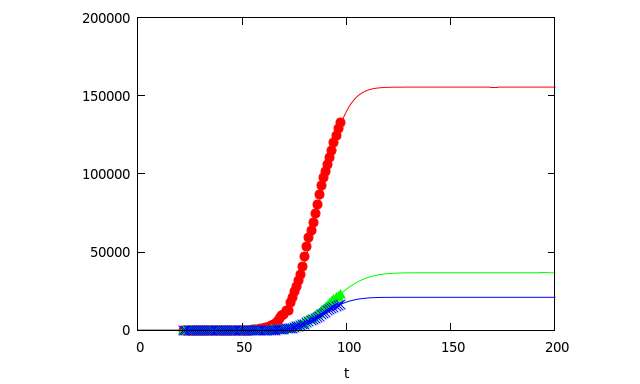
\includegraphics[width=.8\textwidth]{Italy.png}
    \caption{Szenario für Italien (60.4 Mio. Einwohner)}
  \end{center}
\end{figure}
\begin{figure}
  \begin{center}
  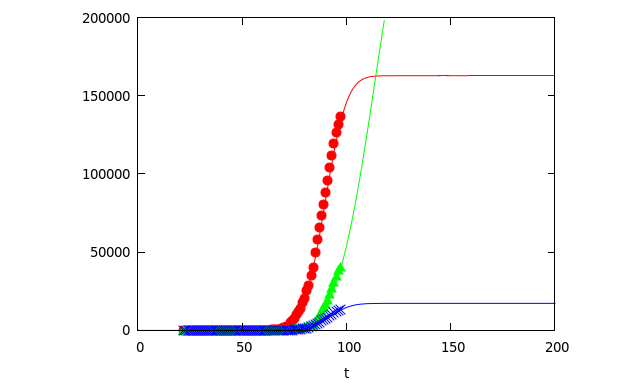
\includegraphics[width=.8\textwidth]{Spain.png}
    \caption{Szenario für Spanien (46.7 Mio. Einwohner)}
\end{center}
\end{figure}

\begin{figure}
  \begin{center}
  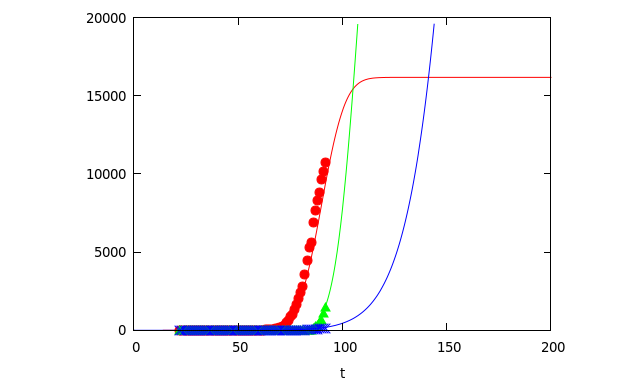
\includegraphics[width=.8\textwidth]{Austria.png}
    \caption{Szenario für Österreich (8.85 Mio. Einwohner)}
\end{center}
\end{figure}

\end{document}
